\section{Finding interchange-consistent Subsets}
\label{sec:method}

Given a causal abstraction candidate \((\mathcal L,\mathcal H,\Pi)\) and an input space \(\mathcal I\), we aim to identify regions of the input space on which the abstraction is fully faithful. Rather than summarizing abstraction quality with a single global IIA score, we seek a more structured view: which inputs are well interpreted by the current hypothesis, which are not, and how this distinction can be used to improve the hypothesis itself. This section proceeds in two parts. Section~\ref{subsec:defining-perfect} formalizes interchange consistency at the level of input pairs and input subsets, yielding a graph-theoretic view of abstraction success and failure \citep{geiger-etal-2020-neural,pislar2025combining}. Section~\ref{subsec:diagnosis-pipeline} then introduces a practical four-step diagnosis pipeline based on this structure to partition the input space and generalize the result beyond the analyzed sample.

\subsection{interchange-consistent Input Subset and the Interchangeability Graph}
\label{subsec:defining-perfect}

Causal abstractions are typically evaluated using interchange intervention accuracy (IIA). Given a causal abstraction \((\mathcal L,\mathcal H,\Pi)\) and a finite set of input pairs \(\mathcal P\), IIA is the proportion of pairs \((i_1,i_2)\in\mathcal P\) for which the low-level intervention matches the corresponding high-level counterfactual for every variable in \(\mathcal H\) (i.e., \(X\in\mathsf{Var}(\mathcal H)\)):
\begin{align*}
\tau\!\left( \text{II}(\mathcal L,i_1,\pi_X)(i_2)\right)
&=
\text{II}\!\left(\mathcal H,\tau(i_1),X\right)\!\left(\tau(i_2)\right).
\end{align*}
While IIA is a useful global summary, it does not reveal how abstraction failures are distributed over the input space. To move beyond a single scalar score, we define a pairwise notion of exact success under interchange interventions and then lift it to subsets of inputs.
\begin{definition}[Interchange-Consistent Pairs]
\label{def:perfect-pairs}
Given a causal abstraction \((\mathcal L,\mathcal H,\Pi)\) and an input set \(\mathcal I\), two inputs \(i_1,i_2\in\mathcal I\) are \emph{interchange-consistent} under \((\mathcal L,\mathcal H,\Pi)\), denoted \(\mathbf p_{(\mathcal H,\mathcal L,\Pi)}\langle i_1,i_2\rangle\), iff for all \(X\in\mathsf{Var}(\mathcal H)\),
\begin{equation*}\label{eq:perfect}
\begin{split}
\tau\!\left( \text{II}(\mathcal L,i_1,\pi_X)(i_2)\right)
&=
\text{II}\left(\mathcal H,\tau(i_1),X\right)\!\left(\tau(i_2)\right),\\
\tau\!\left( \text{II}(\mathcal L,i_2,\pi_X)(i_1)\right)
&=
\text{II}\left(\mathcal H,\tau(i_2),X\right)\left(\tau(i_1)\right).
\end{split}
\end{equation*}
\end{definition}

Definition~\ref{def:perfect-pairs} requires exact counterfactual agreement in both directions: patching from \(i_1\) into \(i_2\), and from \(i_2\) into \(i_1\). We then lift this pairwise notion to subsets.

\begin{definition}[Interchange-Consistent Input Subset]
\label{def:perfect-subspace-method}
An input subset \(I \subseteq \mathcal I\) is \emph{interchange-consistent} by \((\mathcal L,\mathcal H,\Pi)\) iff for all \(i_1,i_2\in I\), \(\mathbf p_{(\mathcal H,\mathcal L,\Pi)}\langle i_1,i_2\rangle\) holds.
\end{definition}

Since we aim to find (quasi-)interchange-consistent input subsets\footnote{In our experiments, we usually search for quasi-interchange-consistent or \(\gamma\)-interchange-consistent input subsets rather than strict interchange-consistent subsets. A subset \(S\subseteq\mathcal I\) is \(\gamma\)-interchange-consistent if at least a \(\gamma\) proportion of input pairs in \(S\) are interchange-consistent. This relaxation reduces computational cost and avoids returning only trivially small subsets when a few failed interventions break an otherwise coherent high-faithfulness region.} we refer to the resulting subsets as \emph{target buckets}, we also refer to such subsets as \emph{target buckets}. This setwise notion naturally admits a graph-theoretic reformulation.

\begin{definition}[Interchangeability Graph]
\label{def:interchangeability-graph}
Given a causal abstraction \((\mathcal L,\mathcal H,\Pi)\) and an input set \(\mathcal I\), the \emph{interchangeability graph} is an undirected graph \(G=(V,E)\) with \(V=\mathcal I\). An edge connects two distinct vertices \(i_1,i_2\in V\) iff \(\mathbf p_{(\mathcal H,\mathcal L,\Pi)}\langle i_1,i_2\rangle\) holds.
\end{definition}

The interchangeability graph provides a map of where a candidate abstraction succeeds. A subset \(I\subseteq \mathcal I\) is interchange-consistent iff every pair of vertices in \(I\) is connected by an edge; in graph-theoretic terms, such a subset is a clique.

\begin{definition}[Clique and Maximum Clique]
\label{def:clique}
A set of vertices \(C\subseteq V\) in an undirected graph \(G=(V,E)\) is a \emph{clique} if every pair of vertices in \(C\) is connected by an edge. A \emph{maximum clique} is a clique of the largest possible size in \(G\).
\end{definition}

One immediate consequence is that a subset \(I\subseteq \mathcal I\) is interchange-consistent by \((\mathcal L,\mathcal H,\Pi)\) iff \(I\) forms a clique in the Interchangeability Graph. This reformulates the search for an exactly faithful region of the input space as a graph problem. 

%In practice, however, strict cliques can be brittle under representational noise, so in the next subsection we introduce a diagnosis pipeline that relies operationally on dense graph structure, rather than insisting on exact maximal cliques.

\subsection{The Diagnosis Pipeline}
\label{subsec:diagnosis-pipeline}

We present a four-step diagnosis pipeline for turning a non-perfect causal abstraction into a more informative object of analysis. The central idea is to move from a single global IIA score to a partition of the input space: rather than asking only whether a hypothesis works on average, we ask where it works, where it fails, and what distinguishes the two regions. The pipeline is task-agnostic, but to make each step concrete, we illustrate it with a running toy logic example (Fig. \ref{fig:logic-task-first-pass}). We use this example here only to show how a \emph{single} diagnosis pass works for one target variable; in Section~\ref{sec:logic-task-recursive}, we return to the same task and show how recursively reapplying the pipeline can recover a fuller high-level hypothesis. The complete diagnosis algorithm is shown in \cref{alg:diagnosis} in the appendix. 

% \begin{figure}[ht]
% \centering
% 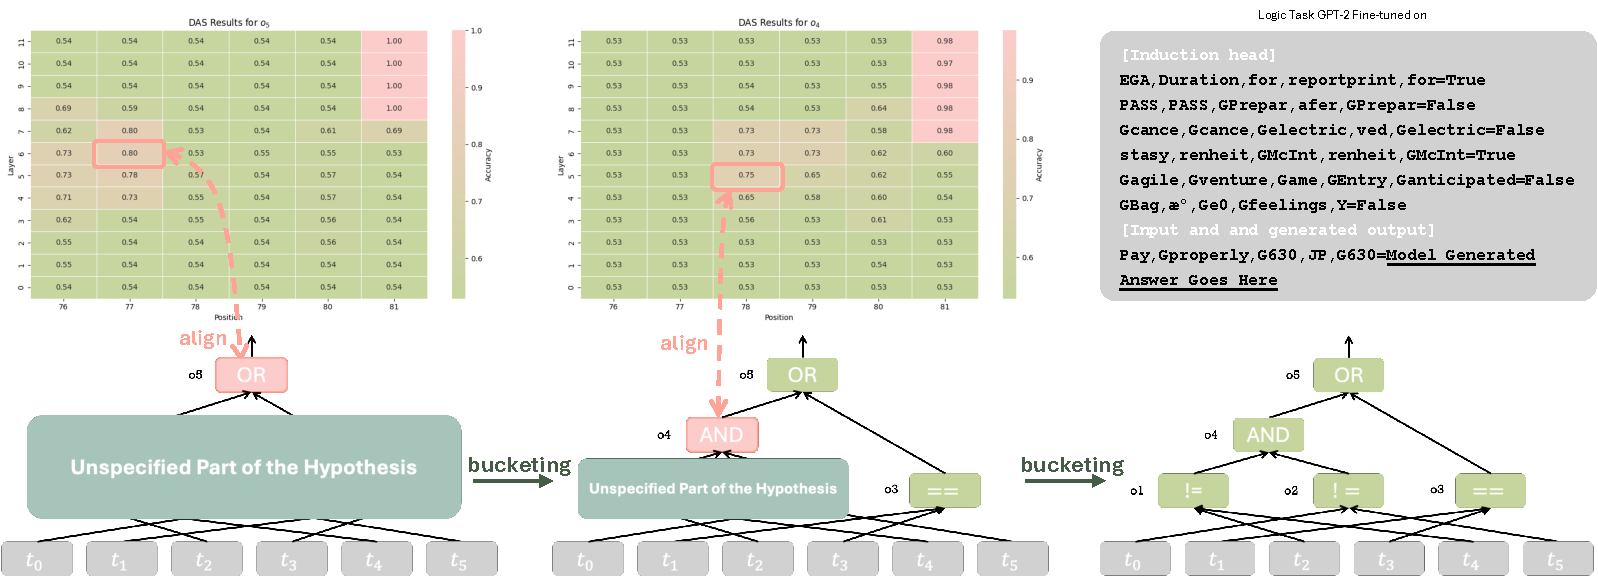
\includegraphics[width=\linewidth]{figs/logic_task.pdf}
% \caption{\textbf{Running example -- a toy logic task.} To illusrate the diagnosis pipeline, we consruct a synthetic logic task. We fine-tune a 12-layer GPT-2-small model to perform a Boolean reasoning task over six input tokens \(t_0,\dots,t_5\). The model is trained to predict a binary label \(o_5 \;=\; \bigl((t_2 \neq t_4)\wedge (t_0 \neq t_5)\bigr)\;\vee\;(t_1 = t_3).\)
% For clarity, we name the intermediate variables \(o_1 := (t_2 \neq t_4),\ o_2 := (t_0 \neq t_5),\ o_3 := (t_1 = t_3) 
% \). The model is trained only on input-output pairs, not on this symbolic decomposition. This means the model can use different computations to get the same correct result (e.g., $y = (o_1 \wedge o_2) \vee o_3$ vs. $y = (o_1 \vee o_3) \wedge (o_2 \vee o_3)$). Therefore, the task serves as a clean testbed for asking which computation the model is actually using to solve the task.}
% % {A GPT-2-small model is trained to predict the truth value of \(o_5=(o_1\wedge o_2)\vee o_3\). Starting from an underspecified high-level hypothesis containing only the output variable \(o_5\), DAS identifies an earlier candidate alignment with non-perfect IIA. Applying the diagnosis pipeline reveals that this alignment is faithful only on the subspace where the conjunction branch \(o_4=o_1\wedge o_2\) is inactive, thereby identifying \(o_4\) as a missing intermediate variable in the coarse hypothesis.}
% \label{fig:logic-task-first-pass}
% \end{figure}

\begin{figure}[t]
    \centering
    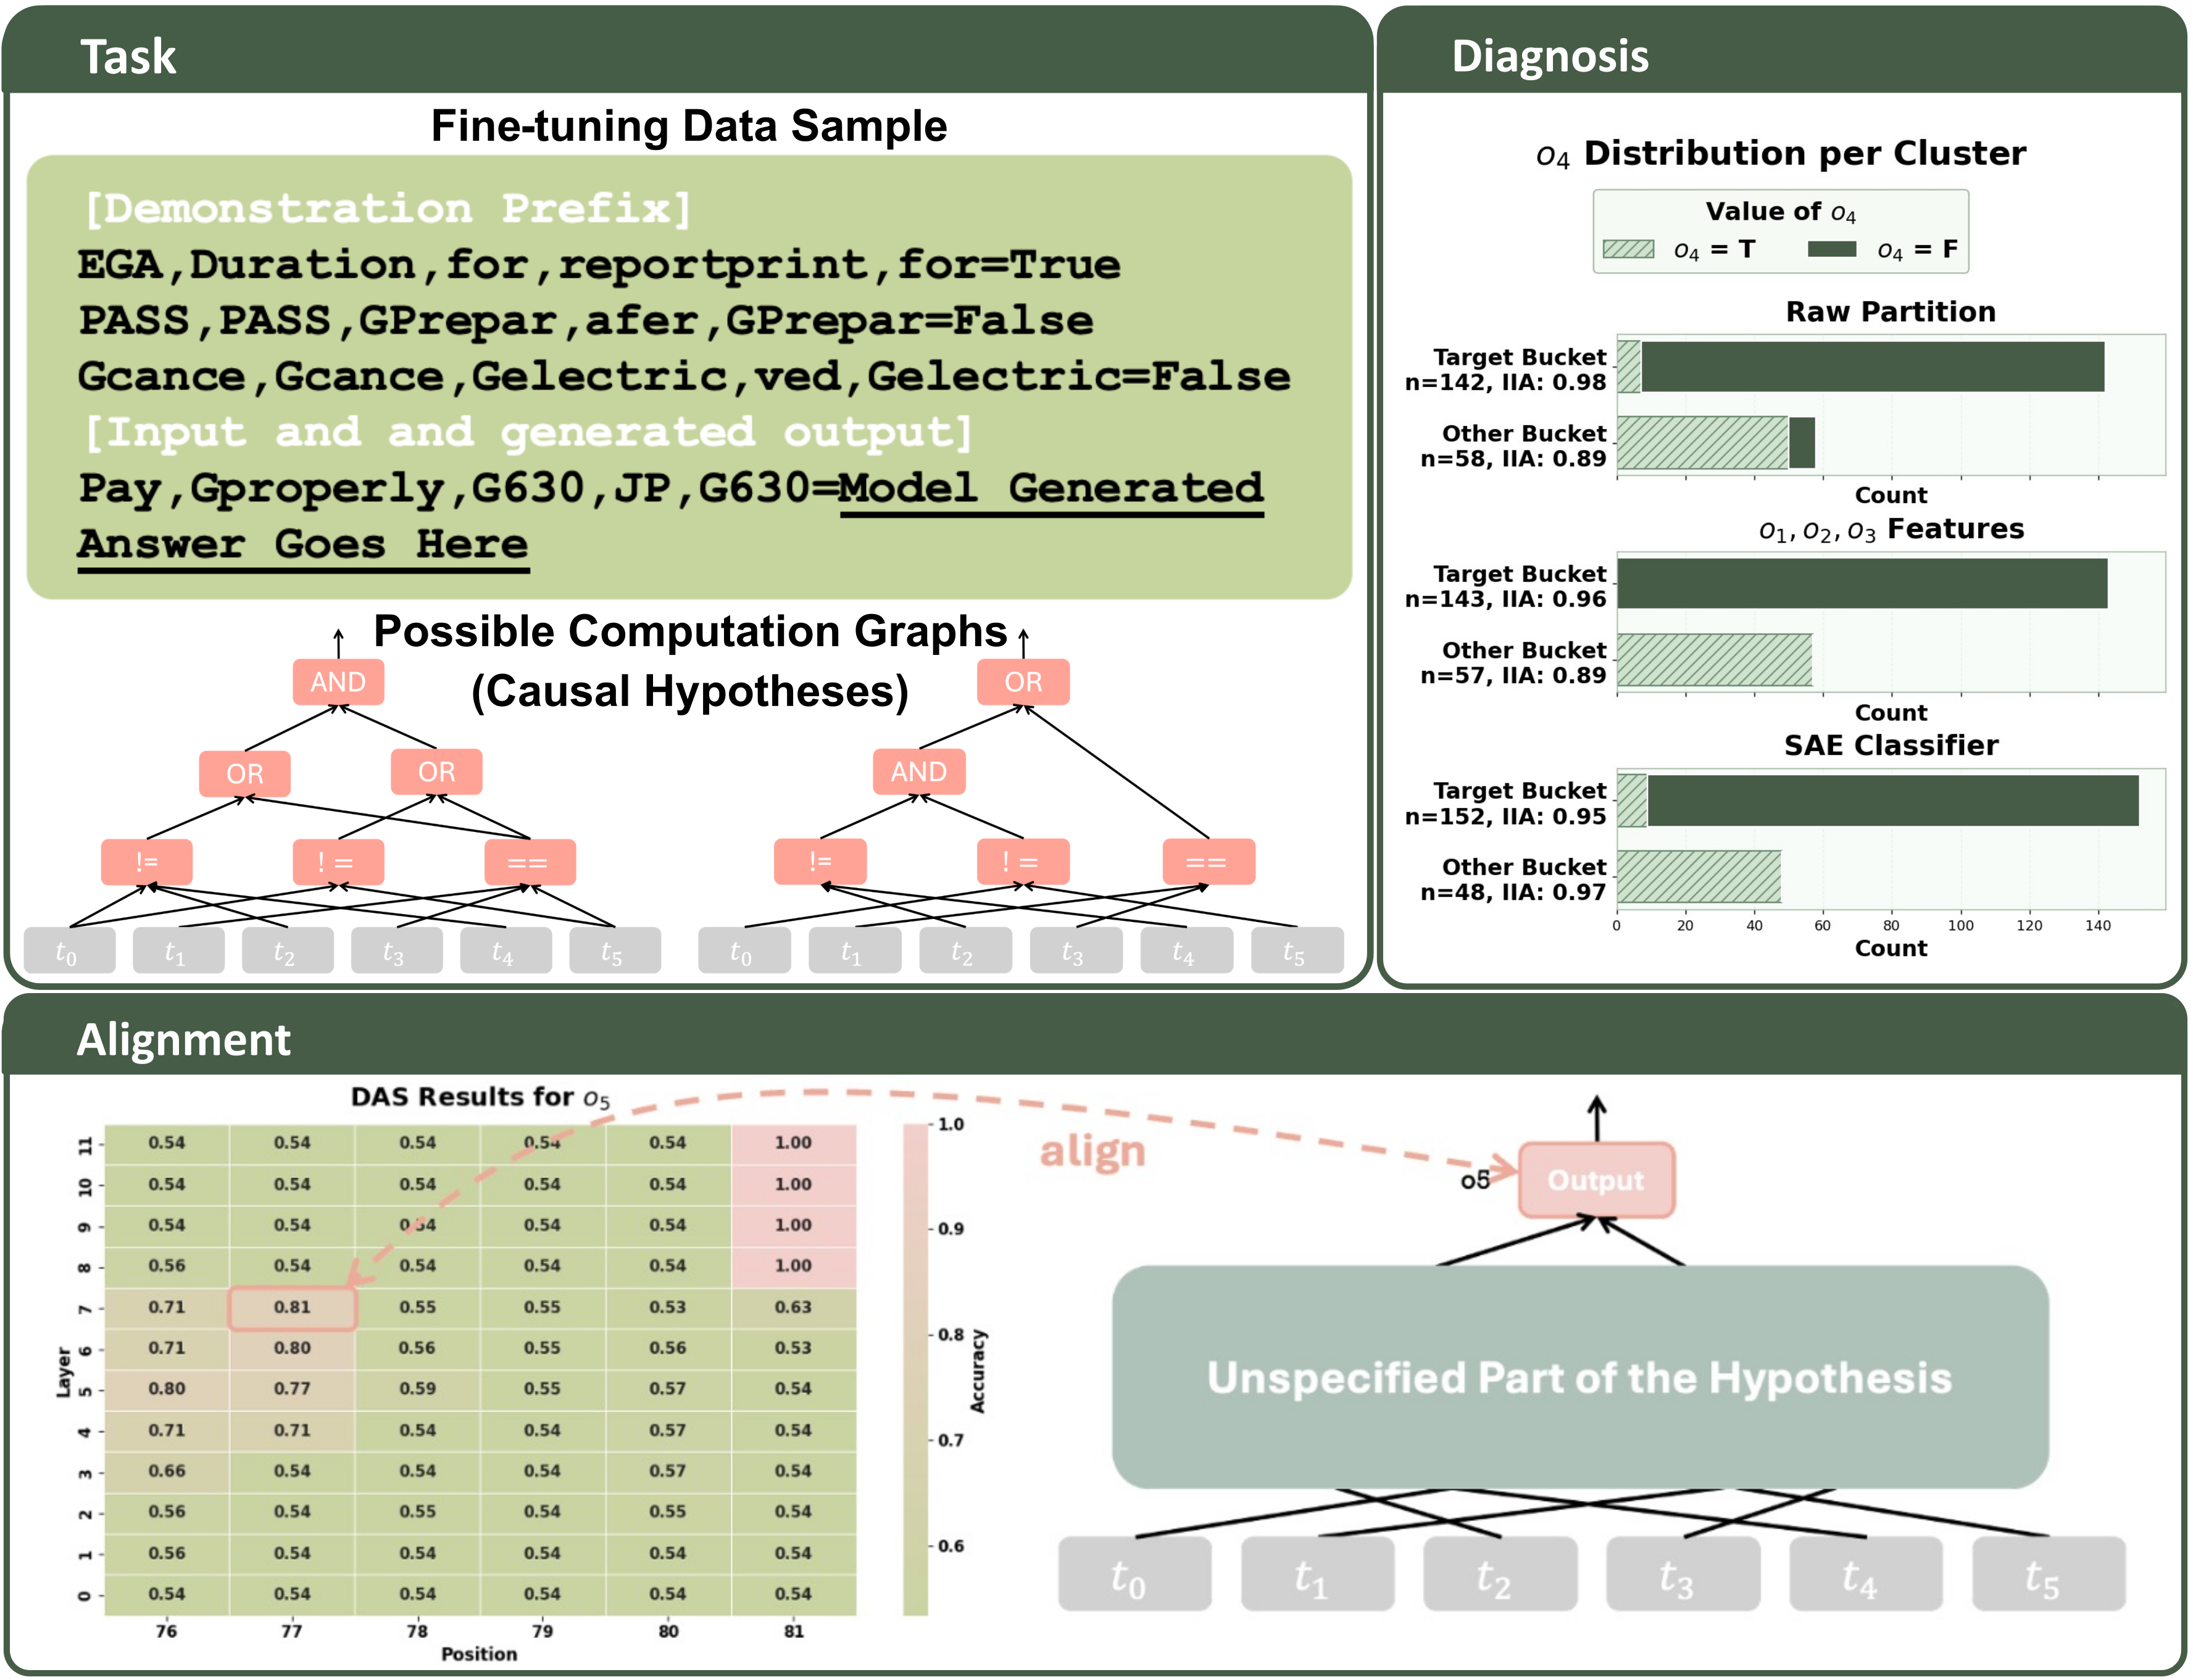
\includegraphics[width=.85\linewidth]{figs/logic_task_new.png}
    \caption{\textbf{Running example -- a toy logic task.} We fine-tune a 12-layer GPT-2-small model to predict the truth value of \(o_5=((t_2\neq t_4)\wedge(t_0\neq t_5))\vee(t_1=t_3)\). For exposition, we denote the primitive Boolean variables (the (non)equalities) by \(o_1,o_2,o_3\), so that the target computation can be written as \(o_5=(o_1\wedge o_2)\vee o_3\). The model is trained only on input-output pairs. This means the model can use different computations to get the same correct result (e.g., $y = (o_1 \wedge o_2) \vee o_3$ vs. $y = (o_1 \vee o_3) \wedge (o_2 \vee o_3)$). Therefore, the task serves as a clean testbed for asking which computation the model is actually using to solve the task.}
    \label{fig:logic-task-first-pass}
\end{figure}

% \begin{figure}[ht]
% \centering
% 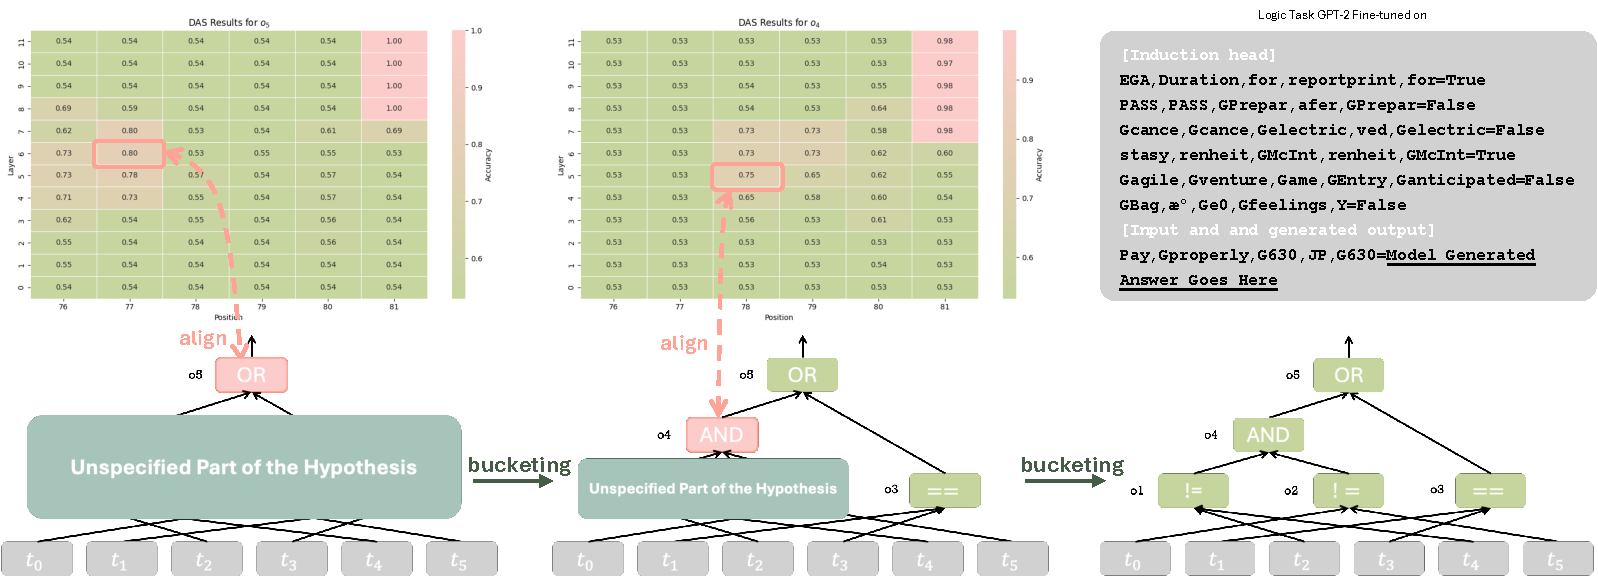
\includegraphics[width=\linewidth]{figs/logic_task.pdf}
% \caption{\textbf{Running example: a toy logic task.} We fine-tune a 12-layer GPT-2-small model to predict the truth value of \(o_5=((t_2\neq t_4)\wedge(t_0\neq t_5))\vee(t_1=t_3)\). For exposition, we denote the primitive Boolean variables by \(o_1,o_2,o_3\), so that the target computation can be written as \(o_5=(o_1\wedge o_2)\vee o_3\). The model is trained only on input-output pairs, not on this symbolic decomposition. This means the model can use different computations to get the same correct result (e.g., $y = (o_1 \wedge o_2) \vee o_3$ vs. $y = (o_1 \vee o_3) \wedge (o_2 \vee o_3)$). Therefore, the task serves as a clean testbed for asking which computation the model is actually using to solve the task.}
% \label{fig:logic-task-first-pass}
% \end{figure}

\textbf{Step 1: Specify the task and the input space.}
The first step of the pipeline is to define a task and an input space \(\mathcal I\) on which the low-level model \(\mathcal L\) performs reliably. This isolates failures of \emph{interpretation} from ordinary task failures. In practice, we therefore restrict attention to the subset of correct predictions: $\mathcal I_{\mathrm{correct}}
\;=\;
\{\, i \in \mathcal I \;:\; \mathcal L(i)\ \text{is task-correct}\,\}.$

\textit{Example:} In the toy logic task, we fine-tuned the model on a generated dataset of size \(20,000\), where \(o_1,o_2,o_3\) are each true with probability \(0.5\). The model achieves \(99.7\%\) test accuracy. We filtered out all the failure cases, and the input space consists of all instances where the model correctly predicts the truth value of \(o_5\). 

\textbf{Step 2: Find a candidate alignment.}
Next, given a high-level variable \(X\), we identify a candidate alignment \(\pi_X\) between \(X\) and an intervenable low-level feature. This can be done using any standard alignment-search method, such as DAS or full-vector patching. At this stage, global IIA provides only a preliminary signal: if it is near-perfect, the hypothesis may already be adequate; if it is at chance, the candidate alignment is likely uninformative; but if it is intermediate, the result will need some further investigation.

\textit{Example:} We deliberately begin from an underspecified high-level hypothesis containing only the final output variable \(o_5\). DAS finds a near-perfect alignment at the final output position, but also an earlier candidate alignment at position \(77\), layer \(7\), with IIA approximately \(0.78\). This is precisely the kind of intermediate result that motivates diagnosis: it is clearly above chance, yet far from sufficient to claim a globally faithful encoding of \(o_5\).

\textbf{Step 3: Bucket the input space by interchangeability.}
We then ask whether a non-perfect alignment is faithful on some \emph{subset} of the input space. To answer this, we construct the interchangeability graph over \(\mathcal I_{\mathrm{correct}}\), where two inputs are connected when they are interchange-consistent under the candidate abstraction. Rather than insisting on an exact maximum clique, in practice, we may relax the fully connected requirement and search for $\gamma$-quasi-cliques, which are subgraphs that have density larger than $\gamma$. We choose $\gamma = 0.98$ in all experiments. We treat the dense quasi-clique as the ``target bucket'' and treat the remainder as ``other bucket''. See Appendix~\ref{appendix:method} for details of the bucketing algorithm.

\textit{Example:} Applying this step to the candidate \(o_5\) alignment reveals that the alignment is not merely noisy. The well-interpreted bucket is dominated by inputs for which \(
o_1 \wedge o_2 = \mathrm{False}\), so that the target computation simplifies to \(o_5 = o_3\). On this subspace, a feature that tracks only the \(o_3\) branch can still appear faithful to the full output variable. By contrast, the under-interpreted bucket is dominated by inputs for which \(o_1 \wedge o_2=\mathrm{True}\), where that simplification no longer holds. The diagnosis therefore localizes a specific failure mode of the coarse output-only hypothesis.

\textbf{Step 4: Generalize and characterize the partition.}
Finally, we train a classifier \(g:\mathcal I \to \{1,\dots,K\}\) to predict bucket membership for unseen inputs. The input to the classifier is a feature representation of each input, which can either be hand-labeled features describing the input, or model-internal features such as SAE, activations, or attribution-based features at the aligned site. The output is a bucket label indicating which bucket the input belongs to. This step serves two purposes: it tests whether the discovered buckets reflect a genuine structural boundary rather than an artifact of a finite intervention graph, and it helps characterize that boundary in terms of the features that best predict membership.

\textit{Example:} In the toy logic task, after bucketing the input space, we train two classifiers using bucket membership as the label. One takes the truth values of \(o_1,o_2,o_3\) as hand-labeled input features, and the other takes SAE features at the aligned position as model-internal input features. Both classifiers can predict the membership of unseen inputs, and their predictions are largely consistent. This indicates that the discovered partition reflects a stable structural distinction, and in particular that membership is indeed governed by whether the conjunction branch \(o_4=o_1\wedge o_2\) is active.

% \textbf{Step 4: Generalize and characterize the partition.}
% Finally, we train a classifier \(g:\mathcal I \to \{1,\dots,K\}\) to predict bucket membership for unseen in-distribution inputs. This serves two purposes. First, it tests whether the discovered partition reflects a genuine structural boundary rather than an artifact of a finite intervention graph. Second, it characterizes the boundary in terms of interpretable or model-internal features, turning the partition itself into a refinement signal.

% \textit{Example:} In the toy logic task, a classifier trained on the discovered buckets reveals that membership is indeed governed by whether the conjunction branch \(o_4=o_1\wedge o_2\) is active. This suggests that the initial output-only hypothesis is missing an intermediate variable corresponding to that branch.

Taken together, these four steps turn a single imperfect IIA score into a structured diagnosis. By deliberately aligning the output variable to a location with an imperfect but above baseline IIA, we identify buckets of inputs with high in-bucket and low cross-bucket IIA. This shows that this alignment is locally faithful within each bucket but collapses distinctions across buckets, indicating that the output variable can be further broken down into two intermediate variables. Figure~\ref{fig:logic-task-first-pass} illustrates this first diagnosis pass on the toy logic task.

% Taken together, these four steps convert a single imperfect IIA score into a diagnosis. Instead of concluding only that a candidate abstraction is partially successful, we obtain a more useful conclusion: it is faithful on one region of the input space, fails on another for a systematic reason, and suggests a concrete refinement to the high-level hypothesis. Figure~\ref{fig:logic-task-first-pass} illustrates this first diagnosis pass on the toy logic task.